
In this section we describe our prototype debugger, CLINT. CLINT embodies the
debugging techniques described in the previous section. In particular, CLINT
consists of three main components: configuration exploration
(\ref{sec:configuration_exploration}), invariant checks
(\ref{sec:invariant_checks}, and cross-layer correlation
(\ref{sec:cross_layer_correlation}).

\colin{Should frame these components as `features we found useful` through specific examples of
bugs they helped us find}

\begin{figure}[t]
    \hspace{-10pt}
    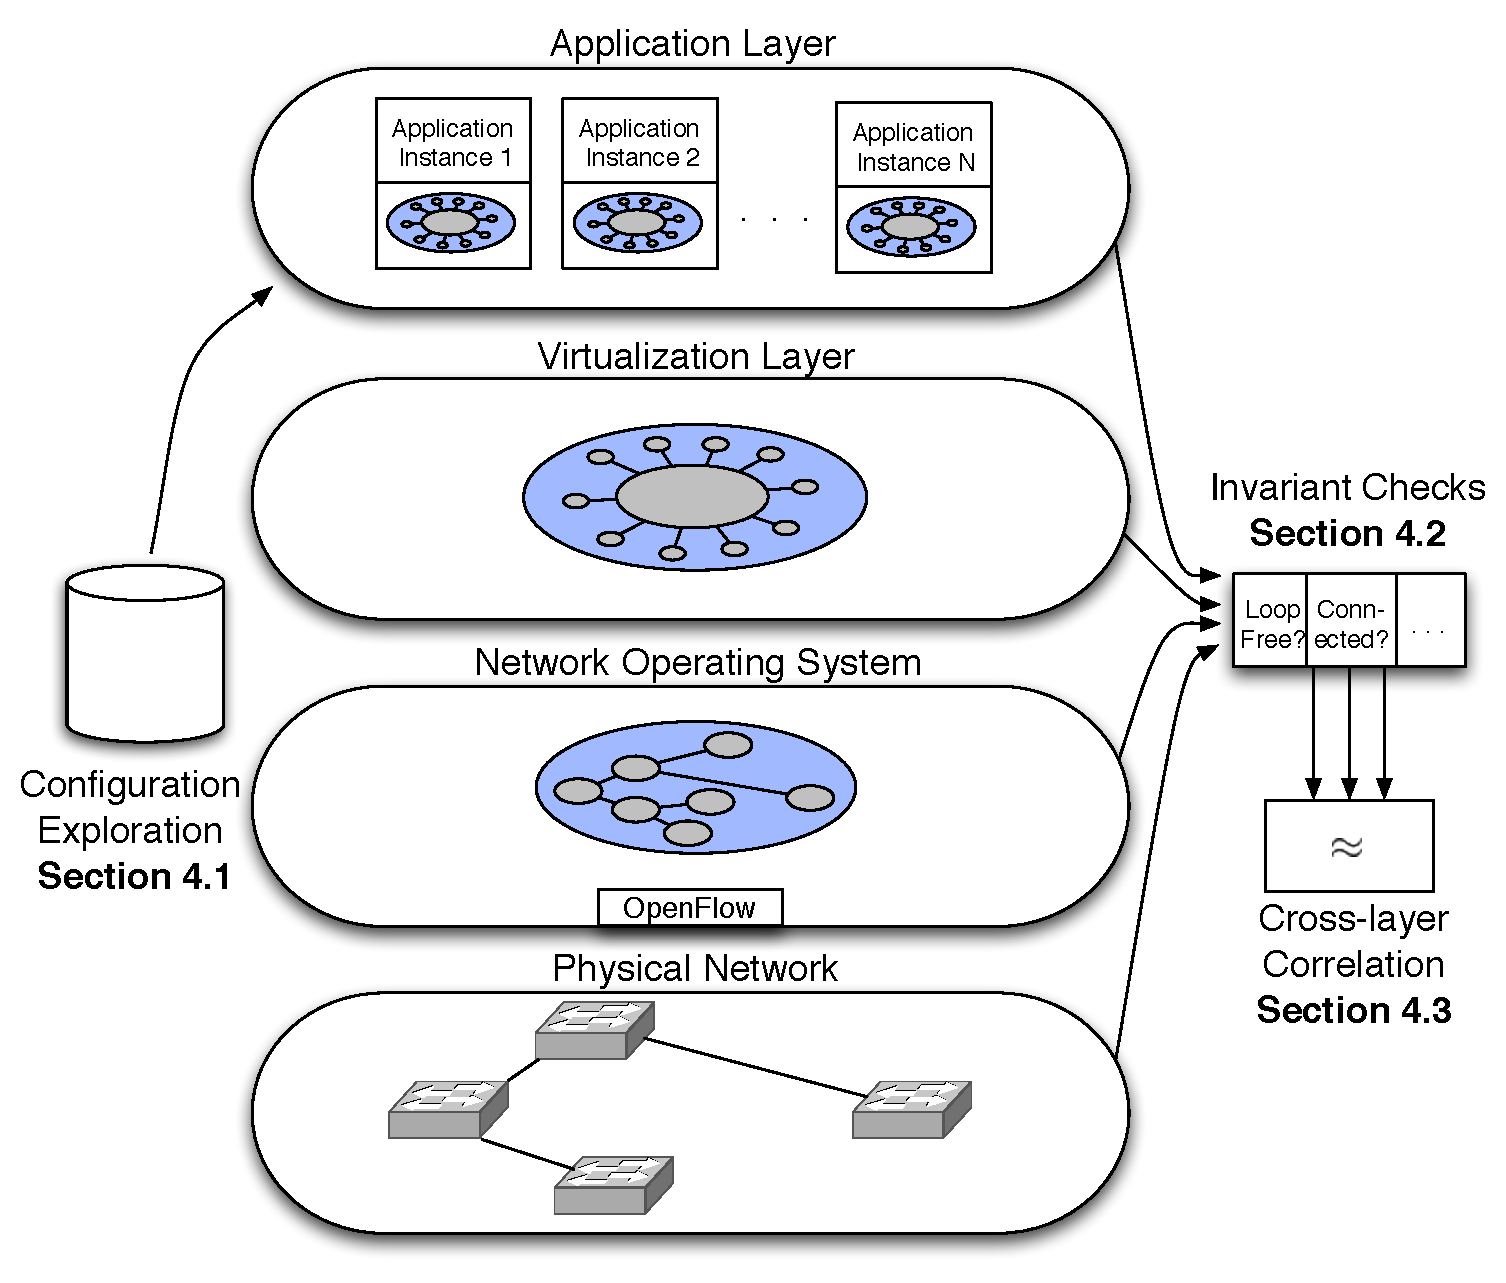
\includegraphics[width=3.25in]{../diagrams/architecture/Architecture_simplified.pdf}
    \caption[]{\label{fig:basicarch} CLINT's architecture. \vspace{-10pt}} 
\end{figure}

\subsection{Configuration Exploration}
\label{sec:configuration_exploration}

High level goal of input generator is to explore the configuration space of
the application. As we move along, feed these output configurations to
Anteater to check for static invariant violations.

\colin{Mention simulation vs. emulation vs. live deployment. Right now we just
have simulation. By running in a single process, we get a global ordering of
events in the system. Later, we'll generalize to truly distributed systems
(at best, can only get a partial ordering of events)}

Right now our system just generates random packets. Later, could be taken from a trace, or
more intellegently chosen (\ie symbolic execution).

Need the replay to be deterministic in order to make it easy to replay the execution
and find the bug.

Execution proceeds in logical rounds. Each round consists of a series of
randomly chosen packet generation events, switch crashes, controller crashes,
packet deliveries, or packet drops. At the end of reach round, we allow the user to
interactively choose the order in which events are executed for that round. We
found this useful for easily reproducing error conditions that a programmer
might have had in mind. \colin{TODO: interactivity isn't actually built yet,
but it would be easy}

\colin{Say something about order-independence. That's what makes the input
generator more than just a mechanism to explore the (static) configuration space}

\subsection{Invariant Checks}
\label{sec:invariant_checks}

At a high level, we essentially run Anteater in a loop. Fuzz, then detect, the
repeat. This helps us i. Explore the entire (static) configuration space of the control
application, and ii. also lets us catch bugs that wouldn't otherwise be
catcheable by Anteater alone. Note that Fuzzer + Anteater is strictly better than Anteater alone.

We use Anteater ~\cite{anteater}! Anteater checks static configurations. We take a snapshot of
the simulated network's state at points specified by the user of the input
generator. Then we feed that snapshot to Anteater, and check whether our
invariants hold.

Particular invariant checks include loop detection, blackhole detection, and
network partition detection. \colin{Maybe routing consistency too, if we
figure out what exactly it means}. 

\subsection{Cross-layer Correlation}
\label{sec:cross_layer_correlation}

At a high level, correspondence checks serve two purposes. First, they help
you isolate the cause of a bug to one particular layer. Second, they ensure
that the network is doing what the application tells it to.

In some sense, it's a global invariant that ``The network should do what the
application tells it to''. In order to verify that this invariant holds, it
does not suffice to check each layer individually. There must be a {\it
correspondance} between each layers' view of the network state.

Check this by translating between each of the layers' representation of the
network state, and verify that there is a one-to-one mapping. 

Virtualization makes this particularly important.

We need to make sure that the translations themselves aren't buggy too! But we
argue that it's far easier to verify corresponance {\it outside} of the system
than it is to write correct code within the virtualization layer itself.

Consistency checks are a subclass of correspondance checks. If you're running
multiple controllers, it must be the case that either: i. The partitioning of
responsibilities betweem the controllers is disjoint, or ii. There is a
correspondance between the controllers' views of the network.

\colin{Virtualization isn't actually a part of POX yet...}
